\chapter{\ifproject%
\ifenglish Project Structure and Methodology\else โครงสร้างและขั้นตอนการทำงาน\fi
\else%
\ifenglish Project Structure\else โครงสร้างของโครงงาน\fi
\fi
}

ในบทนี้จะกล่าวถึงหลักการ และการออกแบบระบบ

\section{หลักการทำงานของแอปพลิเคชัน}
โครงงานนี้เป็นแอปพลิเคชันสำหรับการค้นหาตำแหน่งที่นั่งที่ยังว่างอยู่ภายในสำนักหอสมุดมหาวิทยาลัยเชียงใหม่ พัฒนาขึ้นเป็นรูปแบบเว็บแอปพลิเคชัน
โดยมีการทำงานเริ่มจากกล้องของ ESP32 จะทำการถ่ายภาพ โดยภาพที่ถ่ายจะถูกส่งไปยังคอมพิวเตอร์ที่รอรับภาพจากอุปกรณ์ หลังจากนั้นจะใช้ OpenCV ที่ทำงานร่วมกับ Machine Learning
ในการประมวลผลภาพที่ถ่ายว่ามีคนอยู่ในภาพหรือไม่ หลังจากนั้นจะทำการคำนวณว่าบริเวณนั้นจะมีที่นั่งที่ว่างอยู่กี่ที่นั่ง และข้อมูลดังกล่าวจะถูกส่งไปยังฐานข้อมูล MongoDB เพื่อจัดเก็บข้อมูลแล้วนำข้อมูลดังกล่าว
ไปแสดงผลในหน้าเว็บแอปพลิเคชัน React ในการสร้าง User Interface
\begin{figure}[h]
\centering
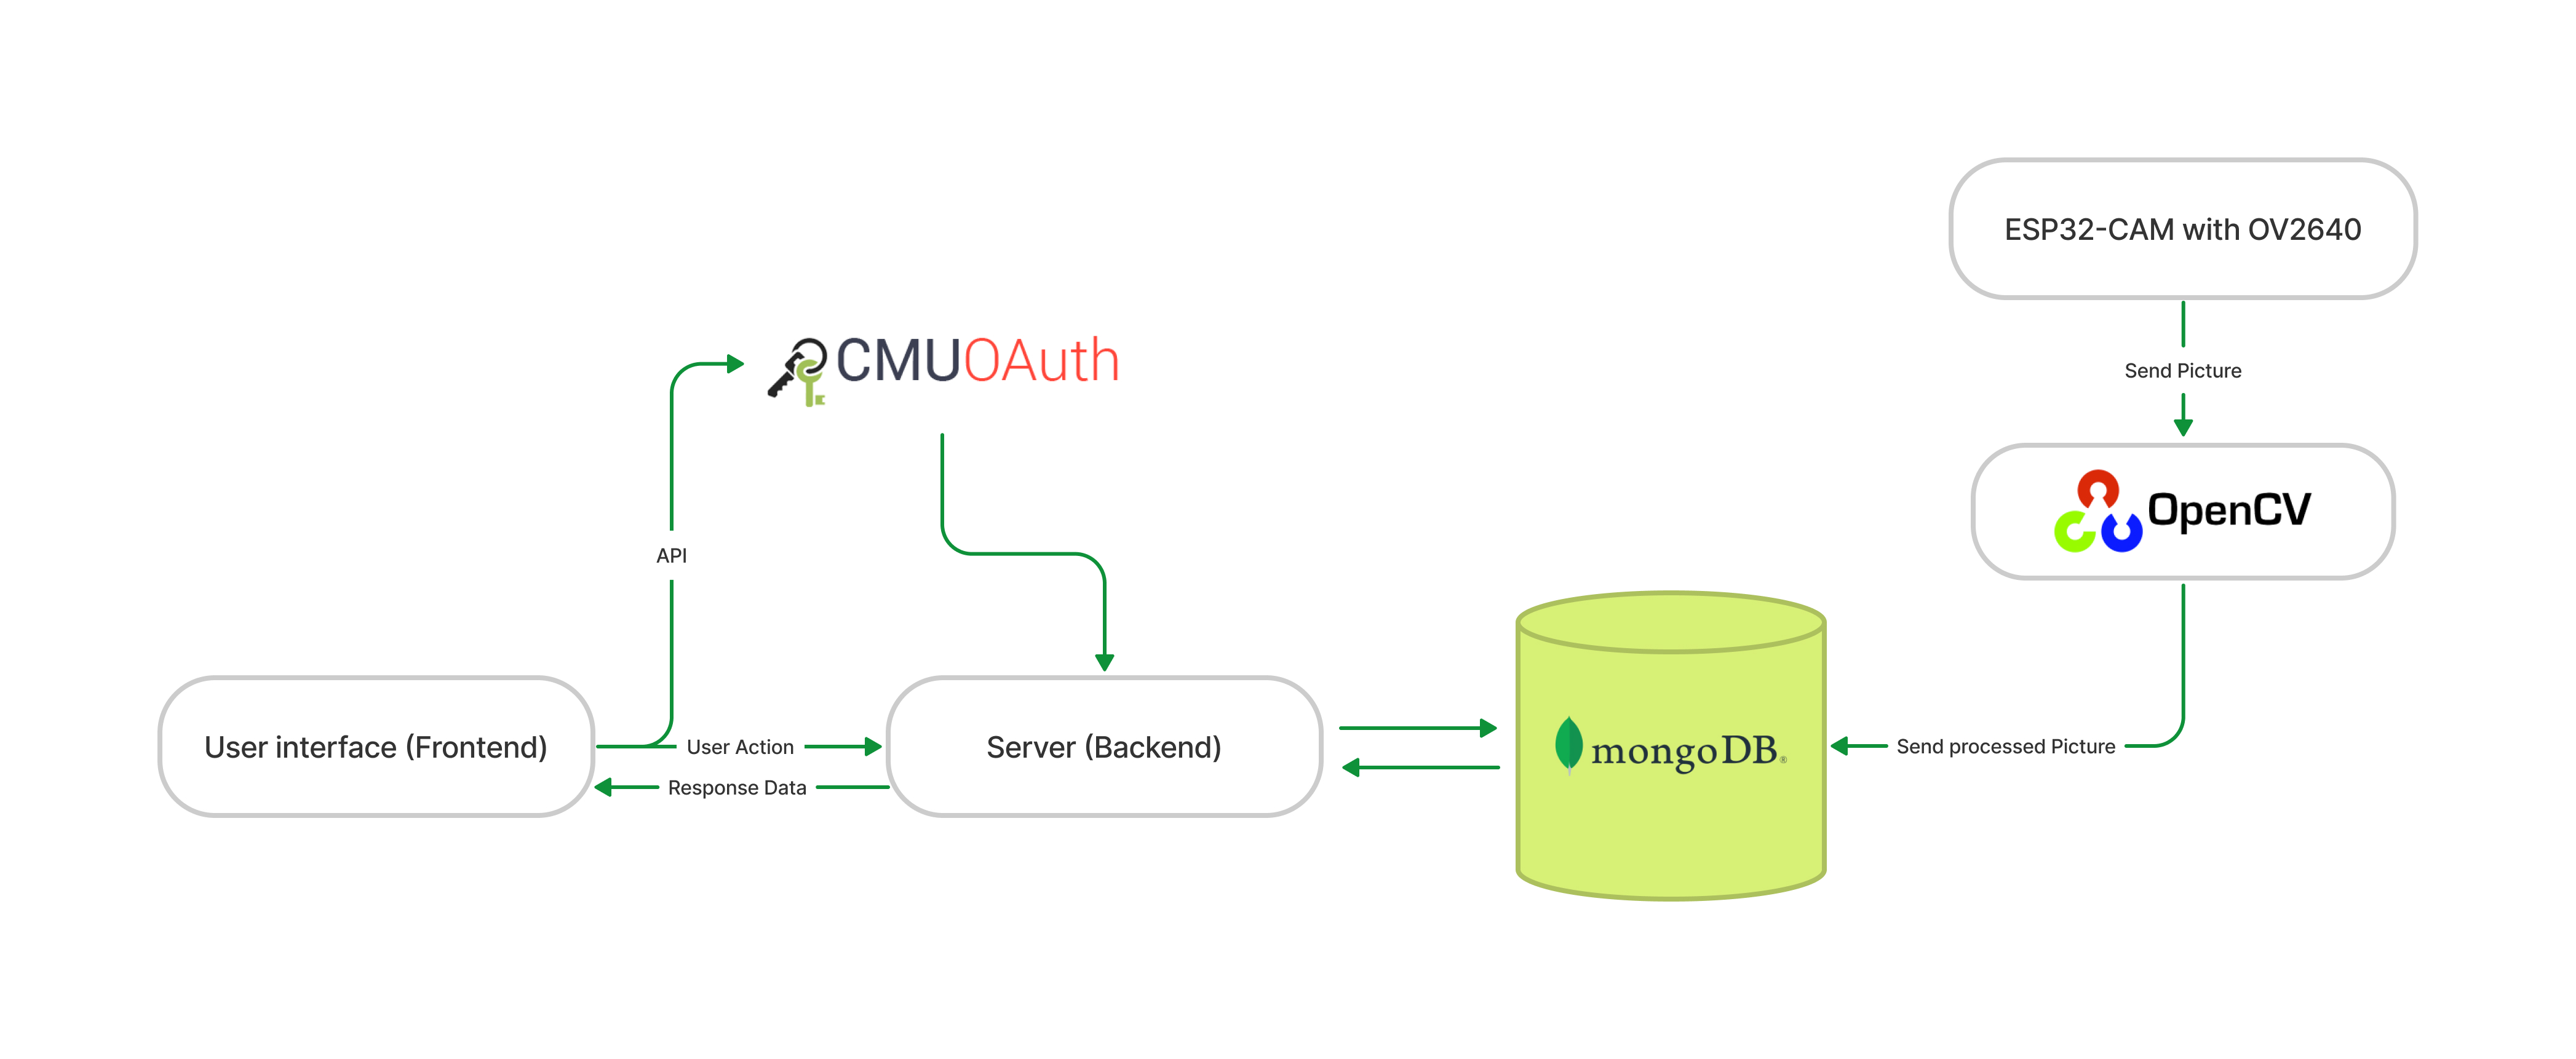
\includegraphics[width=\textwidth]{System Diagram.jpg}
\caption[System Overview]{System Overview}
\label{fig:System}
\end{figure}

\section{การใช้งานของแอปพลิเคชัน}
โครงงานนี้จะแบ่งกลุ่มผู้ใช้ออกเป็น 2 กลุ่ม ได้แก่
\subsection{ผู้ใช้ทั่วไป}
ผู้ใช้ทั่วไปสามารถเข้าใช้งานตัวเว็บแอปพลิเคชันได้โดยไม่ต้องทำการล็อกอินหรือยืนยันตัวตน โดยสามารถเข้าถึงข้อมูลที่แสดงอยู่บน User Interface ได้แก่ จำนวนที่นั่งที่ยังว่างอยู่ จำนวนผู้เข้าใช้บริการในขณะนี้ 
และความหนาแน่นของผู้ใช้บริการหอสมุดในแต่ละช่วงเวลาย้อนหลัง
\subsection{บุคลากรของหอสมุด}
บุคลากรของหอสมุดจำเป็นต้องทำการยืนยันตัวตนผ่าน CMUOAuth เพื่อเข้าใช้งานในส่วนของบุคลากรของหอสมุดโดยข้อมูลที่สามารถเข้าถึงได้จะเหมือนกับกลุ่มผู้ใช้ทั่วไป และข้อมูลที่เข้าถึงได้เพิ่มเติมคือ ความหนาแน่นของผู้ใช้บริการในแต่ละพื่้นที่ย้อนหลัง 
สำหรับนำไปปรับปรุงหอสมุดเพิ่มเติม
